%%
%% Oxford University Press — Bioinformatics
%%
\documentclass[unnumsec,webpdf,contemporary,large]{oup-authoring-template}

% ── Venue flag ────────────────────────────────────────────────────────────────
\newif\ifbiorxiv
\biorxivfalse

% ── Packages ──────────────────────────────────────────────────────────────────
\usepackage[T1]{fontenc}
\graphicspath{{../shared/Fig/}}

% line numbers (uncomment for review)
%\usepackage[mathlines, switch]{lineno}
%\linenumbers

% ── Theorem styles (required by cls) ─────────────────────────────────────────
\theoremstyle{thmstyleone}
\newtheorem{theorem}{Theorem}
\newtheorem{proposition}[theorem]{Proposition}
\theoremstyle{thmstyletwo}
\newtheorem{example}{Example}
\newtheorem{remark}{Remark}
\theoremstyle{thmstylethree}
\newtheorem{definition}{Definition}

\begin{document}

% ── Journal metadata ─────────────────────────────────────────────────────────
\journaltitle{Bioinformatics}
\DOI{10.1093/bioinformatics/xxxxx}
\copyrightyear{2026}
\pubyear{2026}
\access{Advance Access Publication Date: Day Month Year}
\appnotes{Applications Note}
\firstpage{1}

% ── Title ────────────────────────────────────────────────────────────────────
\title[Graph Lens Lite]{Graph Lens Lite: An interactive biological network viewer for displaying, sharing, and exploring disease pathobiology and drug mechanism of action models}

% ── Authors & affiliations ───────────────────────────────────────────────────
\author[1,2,$\ast$]{Matthias Ley\ORCID{0000-0001-6853-8542}}
\author[1]{Kinga Kęska-Izworska\ORCID{0000-0002-4329-1499}}
\author[1]{Lucas Fillinger\ORCID{0000-0001-5341-8097}}
\author[1]{Samuel Walter}
\author[1,2]{Enrico Bono\ORCID{0009-0007-7272-5034}}
\author[1,2]{Louiza Galou\ORCID{0009-0008-5176-2802}}
\author[1]{Peter Andorfer\ORCID{0009-0003-3492-4017}}
\author[3]{Pirmin Hauser}
\author[3]{Johannes Leierer}
\author[1,2]{Klaus Kratochwill\ORCID{0000-0003-0803-614X}}
\author[1,3]{Paul Perco\ORCID{0000-0003-2087-5691}}

\authormark{Ley et al.}

\address[1]{\orgname{Delta4 GmbH}, \orgaddress{\street{Alser Straße 23/30}, \postcode{1080}, \state{Vienna}, \country{Austria}}}
\address[2]{\orgdiv{Division of Pediatric Nephrology and Gastroenterology, Department of Pediatrics and Adolescent Medicine, Comprehensive Center for Pediatrics}, \orgname{Medical University Vienna}, \orgaddress{\street{Waehringer Guertel 18-20}, \postcode{1090}, \state{Vienna}, \country{Austria}}}
\address[4]{\orgdiv{Department of Internal Medicine IV}, \orgname{Medical University Innsbruck}, \orgaddress{\street{Anichstrasse 35}, \postcode{6020}, \state{Innsbruck}, \country{Austria}}}

\corresp[$\ast$]{Corresponding author. \href{email:matthias.ley@delta4.ai}{matthias.ley@delta4.ai}}

\received{Date}{0}{Year}
\revised{Date}{0}{Year}
\accepted{Date}{0}{Year}

% ── Abstract ─────────────────────────────────────────────────────────────────
\abstract{
\textbf{Motivation:} Biological networks are important .. \\
\textbf{Results:} We have developed Graph Lens Lite, a lightweight but powerful interactive network viewer for displaying, sharing, and exploring disease pathobiology and drug mechanism of action molecular models. … \\
\textbf{Availability and implementation:} Graph Lens Lite is available at GitHub (\url{https://github.com/Delta4AI/GraphLensLite}).\\
\textbf{Contact:} \href{mailto:matthias.ley@delta4.ai}{matthias.ley@delta4.ai}\\
\textbf{Supplementary information:} Supplementary data are available at \textit{Bioinformatics}
online.
}

\keywords{Network Viewer, Graph Exploration, Visualization, Drug Mechanism of Action, Disease Pathobiology}

\maketitle

% ── Shared body ──────────────────────────────────────────────────────────────
% shared/content.tex - Body sections shared across all venue flavors.
% Include this from each venue's main.tex after \maketitle.
%
% Convention: venue-specific tweaks use \ifbiorxiv (defined in each main.tex).

\section{Introduction}
Visualization of biological networks is a core technique in systems biology for representation and analysis of complex, often heterogeneous, data. Network visualization combined with quantitative graph analysis such as detection of network modules, hub or bottleneck nodes, or cross-talk between networks can lead to novel hypothesis generation or detection of relevant patterns in biomedical data \citep{ehlersIntroductionSurveyBiological2025}. Biological networks are of particular relevance in digital drug discovery and drug target prioritization and are used in modeling disease pathobiology as well as drug mechanism of action on a molecular level. Biological networks also represent an intuitive way of communicating and sharing research findings with collaborators or disseminating them to the broader scientific community.

Cytoscape and Gephi are considered gold standards for interactive network visualization with an exhaustive plugin ecosystem and rich layout capabilities, but are desktop-focused and lack portability or modern web-app features \citep{shannonCytoscapeSoftwareEnvironment2003,bastianGephiOpenSource2009}. Other tools such as STRING or OmicsNet 2.0 prioritize data integration, enrichment analysis, and access to extensive biological databases over visualization and customization, integrating the network viewer as a helper and not as the focus of the application \citep{szklarczykSTRINGDatabase20252025,zhouOmicsNet20Webbased2022}. Several web-based alternatives have emerged to address portability concerns. Cytoscape Web extends the Cytoscape ecosystem with collaborative workflows for network visualization, though focusing on core functionalities with basic filtering and styling \citep{onoCytoscapeWebBringing2025}. Gephi Lite uses sigma.js for efficient WebGL-based rendering, though it compromises customization, filtering, and advanced styling. Similarly, Graphia provides both a desktop and web client with a powerful 2D/3D rendering engine, but focuses less on user-friendly styling, highlighting, grouping and filtering, prioritizing efficiency, enrichment and layout.

We have developed Graph Lens Lite (GLL) to address the need for a browser-based tool that combines visualization power with an intuitive, streamlined interface, enabling researchers to rapidly explore and evaluate complex networks without requiring expertise in specialized software. GLL offers an expressive query language alongside graphical user interface (GUI)-based filtering, visual grouping, and fine-grained styling controls. Users can compute network metrics, apply customizable layouts, and map data attributes to visual scales. GLL exports networks as portable JSON files that capture the full application state for seamless collaboration, or as data tables for downstream analysis.

\section{Materials and methods}

\begin{figure*}[htpb]
    \centering
    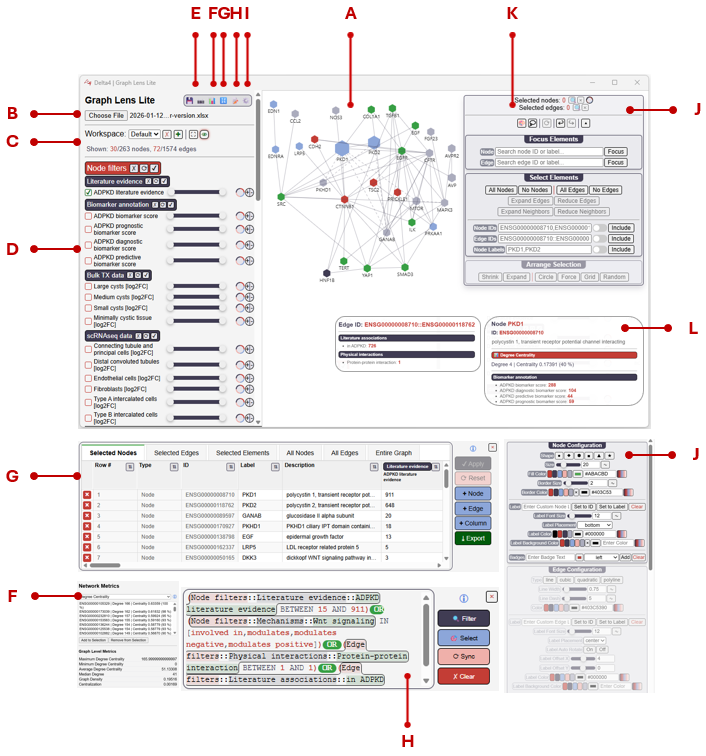
\includegraphics[width=1\textwidth]{main-figure.png}
    \caption{The graphical user interface of Graph Lens Lite. (1) Main network view, (2) File import, (3) Workspace management, (4) Data editor, (5) Query editor, (6) Network and image export, (7) Node and edge filtering, (8) Node and edge tooltip, (9) Network metrics, (10) Selection panel, (11) Style panel, (12) Edit mode.}
    \label{fig:main-figure}
\end{figure*}

\subsection{Installation}
GLL is a free, open-source web application for visualization and exploration of networks. It is written using HTML, CSS, and JavaScript and runs on any modern browser without requiring additional installations. GLL is distributed under the MIT license and its source code is publicly available on GitHub.

\subsection{Data input}
GLL accepts spreadsheets containing node and edge tables, or a JSON format preserving the application state. Input data require an `ID' column for nodes and `Source ID/Target ID' columns for edges. Optional columns may specify visual attributes such as labels, shapes, sizes, colors, or coordinates. Custom properties containing user data can be added as new columns, with optional group labels in square brackets. A template with column specifications, example values, and supported data types is available on GitHub and can be generated from within the application. Additionally, a demo loader enables direct fetching of protein-protein interaction networks from the STRING database \citep{szklarczykSTRINGDatabase20252025}, with plans to extend support to further sources. To support onboarding, the application includes an interactive guided tour that walks users through the interface and its core functionalities.

\subsection{The graphical user interface}
The main GUI elements are shown in Figure 1.

\noindent
\textbf{(1) Main network view:} The central window for displaying and interactively exploring the loaded network. \\
\textbf{(2) File import:} Load files in spreadsheet or GLL JSON format. \\
\textbf{(3) Workspace management:} Save and switch workspaces, reset layout, fit graph to view, and hide disconnected nodes. \\
\textbf{(4) Data editor:} Interactive table for modifying (adding, editing, deleting) nodes and edges and their properties as well as exporting currently filtered nodes and edges. \\
\textbf{(5) Query editor:} Custom query language for nested graph filtering supporting Boolean (AND/OR/NOT), comparison (>=,<=,..), and set-membership (IN [..]) operators. \\
\textbf{(6) Network and image export:} Save the application state to a portable GLL JSON file or export the current view as PNG. \\
\textbf{(7) Node and edge filtering:} GUI-based filtering and visual grouping, synchronized with the query language. \\
\textbf{(8) Node and edge tooltip:} Displays metadata for the selected node or edge elements on click. \\
\textbf{(9) Network metrics:} Controls for computing and applying network metrics to filter and select graph elements. \\
\textbf{(10) Selection panel:} Shows current selection status, lasso selection, and navigation history. An expandable section provides additional focus, search, and layout controls. \\
\textbf{(11) Style panel:} Edit node and edge styles, map parameters and network metrics to visual scales (continuous and discrete color scales, numeric size scales), and customize bubble sets. \\
\textbf{(12) Edit mode:} Fine-grained controls for GUI-based filtering. \\

\subsection{Usage}
\subsubsection{Loading data}
GLL starts by loading network data from spreadsheet files containing node and edge tables (Figure 1.2) or from JSON files. User-supplied properties (coordinates, styling options) are applied where specified. Users can further decide to fetch demo data from the STRING database. The workspace management panel (Figure 1.3) allows switching between independent environments, each preserving its own aesthetics, layouts, filters, and queries.

\subsubsection{Exploring the network}
Once loaded, users can explore the network structure through multiple approaches. The selection panel (Figure 1.10) enables element search, selection, and expansion to connected neighbors. Metadata for selected node and edge elements appear in specific tooltips (Figure 1.8). For deeper analysis, GLL computes topological metrics (e.g., node centrality measures including degree, betweenness, or PageRank) to identify key nodes within the network (Figure 1.9). Users can select a metric and examine one or more highly ranked nodes, with graph-level statistics displayed in the metric panel. In-app documentation describes each metric's methodology and provides references to relevant literature.

\subsubsection{Filtering the network}
GLL supports network filtering through graphical controls (Figure 1.7), with an edit mode for precise input (Figure 1.12), or a query editor for complex operations (Figure 1.5). Node and edge properties can be used for filtering and selection through either interface. The query editor uses a left-to-right syntax and ssupports Boolean operators (AND, OR, NOT), comparison (>=,<=), and set membership (IN) operators, as well as nested conditions using parentheses. Contextual help is accessible via an adjacent icon.

\subsubsection{Styling the network}
The styling panel (Figure 1.11) offers extensive visual customization options for nodes, edges, and groups.  Properties such as geometry (shape, size), color (fill, border, line), labels (text, placement, font), and annotations (badges, halos, arrows) can be configured independently for each element type. Up to four bubble sets allow visual grouping of nodes with adjustable appearance. Numeric and categorical attributes, whether user-supplied or computed from network metrics, can be dynamically mapped to visual features like color and size to highlight importance.

\subsubsection{Editing network data}
GLL includes an integrated data editor (Figure 1.4) for modifying network data in tabular format. Supported operations include column sorting, cell editing, node and edge addition or deletion, table reset, and export to spreadsheet format. Users can also add new columns to define custom properties for nodes or edges, which become immediately available in the filtering and styling interfaces, enabling graph creation and manipulation entirely within the application.

\subsubsection{Exporting results}
A graph can be exported in GLL's native JSON format or as a high-resolution image (Figure 1.6). JSON exports preserve the complete application state, including views, filters, coordinates, and styling, enabling session restoration and collaborative sharing.

\section{Application use case}
\subsection{Visualizing a network-based model of autosomal dominant polycystic kidney disease (ADPKD)}
Autosomal Dominant Polycystic Kidney Disease (ADPKD) is the most common inherited kidney disorder, characterized by the gradual development and enlargement of multiple cysts in both kidneys, which ultimately leads to a progressive deterioration in kidney function \citep{formicaMolecularPathwaysInvolved2020}. ADPKD is a multi-factorial disease involving different disease mechanisms and molecular pathways. The exact mechanisms of ADPKD development and progression are still not fully understood and a better understanding of disease pathobiology is the basis for the discovery of novel drug targets and the development of new treatment options. We consolidated a set of biomedical data on ADPKD to model disease pathobiology and visualize molecular interactions using GLL. Literature associated ADPKD molecular features (genes and proteins) were extracted from Delta4's Hyper-C software platform that consists of sentence-level literature co-annotations between individual molecular features and ADPKD. This set of literature-associated ADPKD molecular features was complemented by genes showing differential expression in ADPKD as compared to healthy tissue based on Omics data. We downloaded the ADPKD bulk RNA-Seq dataset with the accession number GSE7869 from the Gene Expression Omnibus and re-analyzed the dataset to generate lists of differentially expressed genes \citep{songSystemsBiologyAutosomal2009}. Global gene expression profiling was conducted on renal cysts of different volumes, and non-cancerous renal cortical tissue from nephrectomized kidneys were used as controls. Differential gene expression analysis involved data normalization, statistical modeling using linear models, identification of regulated genes based on log2 fold-change (log2FC) and adjusted p-values. Ultimately, the ADPKD phenotype model was enriched with 20 genes which showed absolute log2FC > 2 and adjusted p-values < 0.05 across all four comparisons (large, medium, and small cysts, as well as minimally cystic tissue as compared to healthy tissue from nephrectomized kidneys respectively). In addition we re-analyzed a single-nucleus RNA sequencing (sn-RNA-Seq) dataset with the GEO accession number GSE185948, offering insights into the cellular heterogeneity of ADPKD \citep{mutoDefiningCellularComplexity2022}. Genes with a p-value < 0.05 were included as candidates in the analysis. Ultimately, the ADPKD phenotype molecular model was enriched with genes that were expressed in at least one cell type with absolute log2FC values > 2.5. In addition we retrieved information on genetic associations with ADPKD from the OpenTargets platform \citep{bunielloOpenTargetsPlatform2025}. Expression in healthy tissue and relevant renal cell types of molecular features of the ADPKD molecular model, quantified as normalized transcripts per million (nTPMs), were extracted from the Human Protein Atlas consensus expression profile dataset \citep{karlssonSingleCellType2021}. Information on subcellular location for features of the ADPKD molecular model was retrieved from UniProt \citep{ahmadUniProtWebsiteAPI2025}. Finally, we assigned molecular features of the ADPKD molecular model to mechanisms being discussed in recent reviews to be associated with ADPKD disease development and progression. Assignment of molecular features to mechanisms was done using the Gene Ontology (GO) annotation.

The final constructed ADPKD molecular model consisted of 263 molecular features that were connected by 1574 edges (\textbf{Supplementary datafile S1}). Edges in the constructed network consisted of direct protein-protein interactions consolidated from IntAct \citep{orchardMIntActProjectIntAct2014}, BioGRID \citep{oughtredBioGRIDDatabaseComprehensive2021}, and Reactome \citep{milacicReactomePathwayKnowledgebase2024} as well as of literature sentence-level co-annotations of publications focusing on ADPKD using the catalogs of molecular features and phenotypes as given in Delta4's Hyper-C software platform.

The constructed molecular model can now be used to explore the pathobiology of ADPKD by either filtering for (i) certain molecular mechanisms, (ii) individual cell types, (iii) the most up- or down-regulated genes in renal tissue or specific cell types, (iv) the most central genes based on graph properties like node degree or betweenness among others. Figure 1 for example shows genes of the Wnt signaling pathway (in green for positive modulation of the pathway, red for negative modulation of the pathway, dark blue for modulation of the pathway, and light blue for genes being pathway members without any further information on regulation) as well as additional molecules being associated with ADPKD that are linked to members of the Wnt signaling pathway (in grey) via either protein-protein interactions or co-annotations in the context of ADPKD. This network view allows investigating interesting novel connections of Wnt signaling pathway members with ADPKD-associated proteins.

The molecular model can subsequently also be used to (i) screen for compounds showing beneficial impact on dysregulated disease mechanisms as shown previously in other renal diseases \citep{gebeshuberComputationalDrugRepositioning2023}, (ii) identify drug targets of interest, investigate cell-cell interaction analysis to identify relevant receptor-ligand pairs following previously reported analyses \citep{evgeniouMetaAnalysisHumanTranscriptomics2021}, or (iii) prioritize drug targets for the development of new chemical entities.

\section{Conclusion}
We have developed Graph Lens Lite for visualizing, exploring and sharing biological networks. GLL is designed for portability with a focus on extensive visual customization. The entire application, together with an average sized graph containing approximately 1000 nodes, can be packed into an archive of only a few megabytes. Unlike comparable tools that may require installation, GLL requires only a web browser for core functionality. GLL is distributed as platform-specific Electron bundles for Windows, macOS, and Linux, as well as a platform-independent, self-contained HTML file. This minimal distribution enables users to load demonstration data or create and work with templates without external dependencies or API calls, ensuring long-term stability and offline operation.

\section*{Acknowledgments}
The authors want to thank all working group members of the EU COST Action Program PerMediK (Personalized Medicine in Chronic Kidney Disease: Improved outcome based on Big Data) for fruitful discussions during the regular COST Action project meetings.

\section*{Author contributions}
M.L.: conceptualization; resources; software; visualization; writing - original draft, review \& editing. K.K.-I.: data curation; validation; writing - review \& editing. L.F.: validation; writing - review \& editing. S.W.: validation; writing - review \& editing. F.B.: validation; writing - review \& editing. E.B.: validation; writing - review \& editing. L.G.: validation; writing - review \& editing. P.A.: validation; writing - review \& editing. P.H.: data curation; validation; writing - review \& editing. J.L.: data curation; funding acquisition; validation; writing - review \& editing. P.P.: conceptualization; data curation; funding acquisition; supervision; validation; writing - original draft, review \& editing. K.K.: funding acquisition; supervision; validation; writing - review \& editing.

\section*{Supplementary data}
Supplementary datafile S1: The ADPKD molecular model input file

\section*{Conflict of interest}
K.K. is a co-founder of Delta4 GmbH (Vienna, Austria). M.L., K.K.-I., L.F., S.W., F.B., E.B., L.G., P.A., and P.P. are employed at Delta4 GmbH (Vienna, Austria).

\section*{Funding}
This project has received funding from the Austrian Research Promotion Agency (FFG) under grant agreement number 915133 (ADPKD Drug Discovery). Enrico Bono is supported by a grant from the European Union's Horizon Europe Marie Skłodowska-Curie Actions Doctoral Networks program project PICKED (HORIZON–\allowbreak{}MSCA–\allowbreak{}2023–\allowbreak{}DN-01, grant number 101168626). Louiza Galou is supported by a grant from the European Union's Horizon Europe Marie Skłodowska-Curie Actions Doctoral Networks Industrial Doctorates program project PROMOTE (HORIZON–MSCA–2023– DN-01, grant number 101169245). Paul Perco and Matthias Ley are members of and would like to cordially thank the EU COST Action Program PerMediK, CA21165, supported by COST (European Cooperation in Science and Technology).

\section*{Data availability}
The source code, test data, templates and documentation are available at GitHub (\url{https://github.com/Delta4AI/GraphLensLite}).



% ── Bibliography ─────────────────────────────────────────────────────────────
\bibliographystyle{oup-abbrvnat}
\bibliography{../shared/reference}

\end{document}
